\chapter{Implementation/Tests}
\label{chap:Implementation}

In this chapter I will discuss some of the decisions I have made while
developing the system, and why I made that decision instead of going with
another implementation that was possible.

I will also cover some of the ways I have used the technologies that I chose in
the previous chapter, as well as how they are working together.

In the end I will get a bit into how I have tested the system throughout the
development process, both in regards to unit testing and integration testing.

\section{Entity framework}
\label{sec:Entity framework}
One of the things the entity framework brings is the "repository pattern", as
well as the "Unit of Work pattern". The idea behind those are described in
section~\ref{sec:Patterns}. I however have chosen to wrap them again, so that I
can reduce the dependency to a database implementation and ORM implementation,
in the outer most layer. 

The decision to wrap the implementations also allow me to mock the
implementations a bit easier in some cases when it comes to testing. 

Instead of having a controller call the entity implementations directly, I have
a set of interfaces in the DomainServices layer of the onion model, that I can
use for injection, these interfaces implement my personal implementations of
repositories, and allow me to customize the way I want to deal with the data. 

I have a generic repository, which is capable of doing the most common
operations, such as add a new model to the database, and getting them out again.
It also makes sure to set the right states of the model when I update a model,
and delete one. 

One thing that I use is the idea of telling the repository how I want it to
update the existing model via an action, which it takes as an argument. The
reason for that is it allows me to not update all the properties, but only the
ones that is relevant. Because I only update the relevant ones, if the User of
the program sends in changed data for a property they are not supposed to be
able to change, it will not be changed. 

The generic interface also allows me to implement a standardized way of dealing
with pagination, which is the idea of instead of pulling everything out of a
table, we order the entries, and return a subset of the data. 

This allows the user to ask for ex 10 entries in the table Users, and only get
the 10 entries they asked for. Because they are now not getting all the data
they need to be told how much data there is, and therefore we return the total
number of entries in the search, as well as the page size they got, and the page
they are looking at. The page number is used to set the first entry to the one
with $index = page number \cdot page size$. 

In the simple cases I let the controllers depend on the generic repository, as
there is no need to implement a special handling of cases where no special
update or create logic is needed. But for the cases where we need to link tables
together I have decided to make specific implementations, which themselves
depend on the generic repository, as the logic to save get and update can be
reused, there just needs to be added some more logic on to it. 

I don't have any saving logic in any of the repositories, because I want to be
able to make multiple repository calls in one go, and if any of them fails the
idea of unit of work should step in and make sure that none of the changes take
place. 

Because of this I have implemented a interface to handle the unit of work, with
the ability to call save changes, which all the controllers implement, and use
in the cases where data changes. 

The only place where I don't follow these setups is in the user controller, as
it uses the Identity framework for authentication and authorization, and it
brings its own user manager, which I need to use if I want the feature they
bring. The problem with this user manager is that it does not follow the unit of
work pattern, which means it saves every time I make a call that would update
the database. 

\subsection{Cascade delete}
Some of my connections between entities are many-to-many relations, which for
actual implementation purposes is handled by having a table in between the two
tables, that link them together with a one-to-many relation to both of the
tables. 

Usually you would use the foreign keys as a composite key so there cannot be any
duplicate connection.

Because this can easily create multiple cascade paths on delete, I have decided
to set the entity framework up in such a way that it will not create cascade
deletes on many-to-many relations. 

Because of this I need to manually clear up the relations when I want to delete
an entity that has one, but the manual delete gives more control, and will
therefore not risk creating deletion race conditions, which the problem of
multiple cascade paths result in.

Another thing to notice when looking at the domain models is that I don't
always manually create the many-to-many relation. This is because entity
framework can figure that out itself, assuming i give it the information it
needs. But in some cases namely UserGroups I do make it manually, this is
because it does give me more control over what relations are where, and the
creation of them, even though it makes the code a bit more complex.

\section{Exception filters}
\label{sec:Exception filters}
To be able to return the appropriate response when something fails, I have
decided to throw appropriate exceptions, with messages of what went wrong in
case that is not obvious from the exception itself.

To help with this I have implemented an extension method for getting things out
of the database. If I want to get a single thing out, I would call
SingleOrDefault, but if I need the result to be something, and the default value
therefore is not useful. For this I have implemented the extension function
SingleOrExcept, which just uses SingleOrDefault where if it returns null it
throws a NotFoundException.

To make the response appropriate in the controller I could go with different
approaches. The most basic way of dealing with this would be to catch the
exceptions, and return the right message to the client.

Another way to deal with this is to use filters, this is the way I have decided
to go with. For filters there are still multiple ways to do this, I could have
set the filter on a per method, per controller, or for the entire server.

The implementation of the filter would look like the one of
figure~\ref{fig:notfoundfilter} for all of the types, and since I need the
filters to apply to all the controllers I have gone with the cross project
solution. 

\begin{figure}
  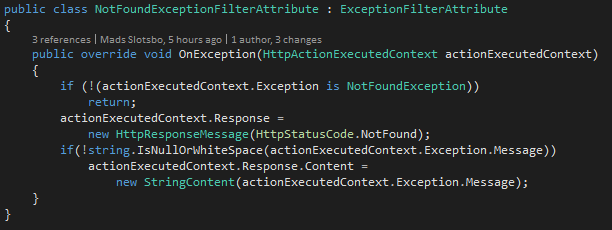
\includegraphics[width=\textwidth]{code/NotFoundExceptionFilterAttribute}
  \caption{NotFoundException filter}
  \label{fig:notfoundfilter}
\end{figure}

\section{Graph data calls}
\label{sec:Graph data calls}
For the data extraction I start by pulling the data out of the database, and
then send it to the method that will format it properly. The reason I do it like
this is that it allows me to use the method no matter where the data comes from. 

I make use of LINQ\footnote{Language-Integrated query} to manipulate the data
since it allows me to group by different keys, and filter away some of the data.

For the production graph, i have two calls, one for the production data, and one
for the goal data. The call for production data is the most interesting, in that
it needs to deal with spacing the earned money out over the period it spans in.

This also means that i had to make a filter that includes the opportunity as
long as it is within the range on the period.

\begin{figure}
  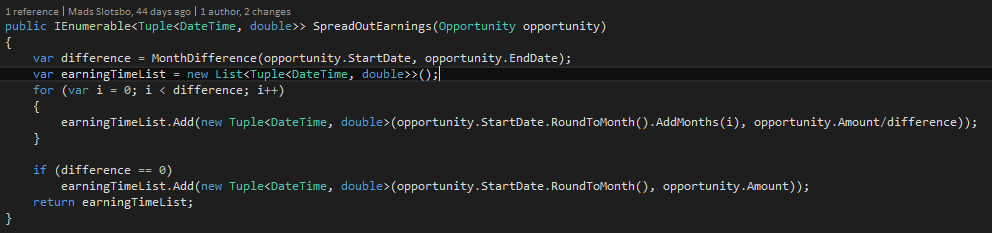
\includegraphics[width=\textwidth]{code/SpreadOutEarnings}
  \caption{SpreadOutEarnings implementation}
  \label{fig:spreadoutearnings}
\end{figure}

In figure~\ref{fig:spreadoutearnings} the implementation of the evening out of
the earnings is illustrated, as can be seen the implementation the result us a
list of tuples. The reason i use tuples here is that it allows me to associate
the earned value with the month it was earned.

When the list is returned I filter away the months that i don't need, based on
the filter, and match it up with a user.

In the end I map the result to a dictionary, with the users email as the key.
The reason I can do that is that the email is unique, and I have grouped them
together ahead of time, to allow me to only have one dictionary entry per user,
containing a list of earnings per month.

\section{Testing}
To separate the testing from the rest of the code I have created a separate
project containing all the automated tests. The advantage of this is that the
tests are not necessarily part of the code that is put on the server that runs
the actual application, but I still have it in the same project, and can
therefore run the tests as required.

\begin{figure}[h]
  \centering
  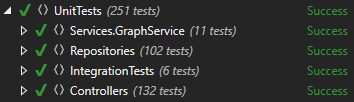
\includegraphics{testResults}
  \caption{Test results}
  \label{fig:testResults}
\end{figure}

The results for all the automated tests can be seen in
figure~\ref{fig:testResults}, where the results are separated into folders, one
for each project, and one folder for the integration tests, as I don't have as
many of those.

To make testing work I have had to create a fake database layer, that implements
the same interface as the real one, allowing me to run the tests against a
nonexistent database, or rather data kept in memory.

The framework I have used for testing is xUnit, which is created by the same
person who created nUnit~\cite{xunit}. The setup for a test is run in the
constructor, and each test is marked either with Fact or Theory, where in theory
the test functions take arguments, and you give it multiple different
combinations of arguments, to run the same test with each.

\subsection{Unit tests}
\label{sec:unit_tests}
Under the development I have created a lot of unit tests, to test that my
functions actually do what i want them to do, and return the correct data.

In figure~\ref{fig:testResults} every test except the ones in the
IntegrationTests folder are unit tests, meaning the test only test a single unit
at a time.

In practise this means that I replace all the dependencies with mocked versions.
For this i have used a mocking framework by the name
NSubstitute\footnote{http://nsubstitute.github.io/}. This is one of the places
where the injection pattern comes in handy, as I can substitute the injected
dependencies with versions that are not real. NSubstitute allows me to control
what specific functions should return or do if they get called, which means i
can know exactly what is going on outside my test when it is run.

An example of substitution of a method could be PersonsControllerTest where I
substitute the IPersonRepository argument to the controller, and later when I
know the controller is going to call a function in that one, such as when I want
to get a single object from the database I can tell the function that it should
return a specific object in that case, as I am not interested in testing the
controllers ability to fetch data, but rather test that it does not mess up the
data, and it actually tries to get it. 

For the case where it fails, the test is more a case of does the controller
catch the exception and act like nothing happened, which is the wrong behaviour
or does it let it go through, and let the filters handle it. In the failing
cases the most interesting tests are the ones where we save to the database, as
we want to make sure that we never make it ca call Save() if something went
wrong, as that puts the database in an unknown state, as mentioned in
section~\ref{sub:unit_of_work_pattern}.

I have tried to keep follow the ideas of test driven development, by writing my
tests first, and making the implementation afterwards, so that the tests work as
a description of what i expect the function to return given specific arguments.

\subsection{Integration tests}
\label{sec:integration_tests}
An integration test is a test that tests a full flow, instead of just testing an
isolated part of the program. The idea of this is to test the communication
between components.

There will automatically be less integration tests than unit tests, as there are
more units in the code than flows. In my case I have not written as many
integration tests as I could have since a lot of the integration testing have
been done manually when writing the front-end, where I have to make the calls for
data to show up in the system, as well as the creation, and manipulation calls.

The unit tests are generally more useful for the development, in that they help
identify where the issue may be in the code, instead of saying that starting
from some point given some arguments something went wrong.

\section{Chapter summary}
For communication with the database I use Entity framework, which is an ORM
allowing me to interact with the entities as if they were C\# objects. This
gives me the advantage of type safety, as well as it allows me to use LINQ which
is a powerful list comprehension library in C\#.

Even though entity framework implements the repository pattern, I have wrapped
it in my own implementation, in order to gain more control, and reduce repeated
code for tasks such as deleting, and and updating. It also allows med to make
better use of injection, in that I can inject a repository interface into a
class, and replace it for testing, so that i can know exactly what information I
am working with.

I make sure to never call save in the repositories, as they are not able to know
if anything else will be happening with the database later in the call, but only
save when the controller decides that it should be done. To make sure that it is
obvious that is the way to do it, I have created a unit of work class, where the
only thing it can do is call save. This way I can also ignore what kind of ORM I
am using for communicating with the data storage entirely in the controllers, as
it is not important here.

In the case a user asks for something that does not exist, eg. an opportunity
with an id that is not in the database, the repository will throw a
NotFoundException, which will propagate all the way outside the controller. The
reason the caller will not get an InternalServerError, is because I use filters,
that catch the exception, and translates it into a not found response. This
filter is applied globally for all the controllers, together with a few others.

The system also works with extracting data so that is can be graphed. This means
that the system pulls out the data based on a filter, and then formats it so
that it is easy to illustrate in a graph or table, and compare each point.

For testing I use xUnit, which allows me to create test methods, that each test
a specific thing. Under the development I created unit tests, so that I could
see if a single bit of the program does what I expected of it. For the unit
tests I made use of the injection, by mocking the dependencies of the class, and
managing the results of the calls the tested method made.

Because there are more smaller units in the application than there are use cases
there are a lot more unit tests than integration tests. This is also because
most of the integration testing has been done via the JavaScript application I
have developed next to the server, which results in the tests not being
automatic, but in order for the JavaScript application to work I the server
still had to work, and the unit tests are there to help identify where the
issues may have shown up.
